\chapter{半导体中的杂质和和缺陷能级}

\section{Si、Ge晶体中的杂质能级}

\subsection{替位式杂质和间隙式杂质}

杂质进入半导体后只能以两种方式存在,一种是杂质原子位于晶格原子间的间隙位置,称为\textbf{间隙式杂质},另一种是杂质原子取代晶格原子位于晶格点处,称为\textbf{替位式杂质}。

间隙式杂质原子一般比较小,如 $\ce{Li+}$半径很小($0.068\ \mathrm{nm}$),在$\ce{Si},\ \ce{Ge},\ \ce{AsGa}$中是间隙式杂质。

形成替位式杂质时,要求杂质原子的大小与被取代的晶格原子大小相近,价电子壳层结构相近。如III、V族元素在IV族半导体元素晶体(Si、Ge)中形成替位式杂质。

单位体积杂质原子数称为\textbf{杂质浓度},通常用于表示半导体晶体杂质含量。

\subsection{施主杂质、施主能级} 

III、V族元素在Si、Ge晶体中形成替位式杂质。

在如\autoref{fig:Ge-As}所示的替位杂质中:
\begin{figure}[ht]
    \centering
        
\tikzset{every picture/.style={line width=0.75pt}} %set default line width to 0.75pt        

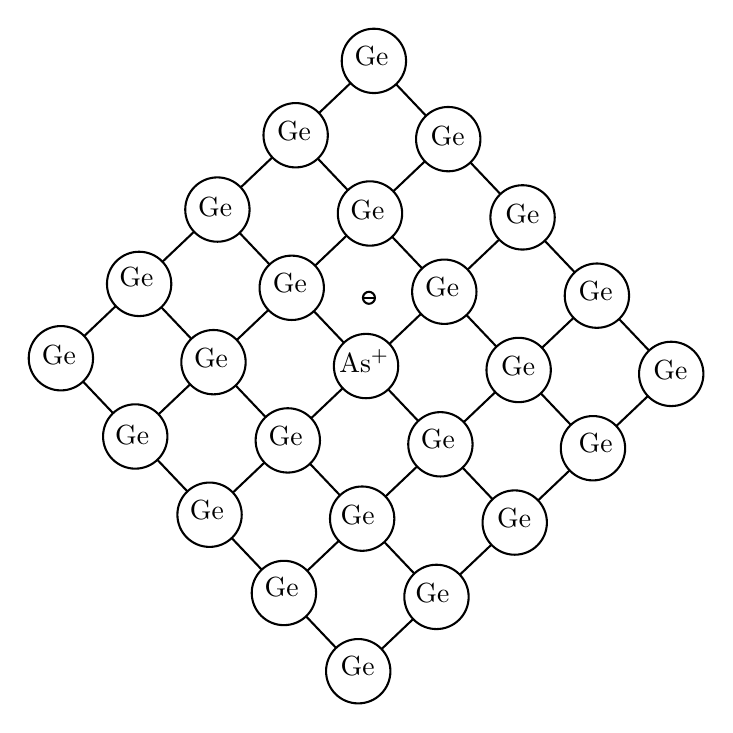
\begin{tikzpicture}[x=0.75pt,y=0.75pt,yscale=-1,xscale=1]
%uncomment if require: \path (0,395); %set diagram left start at 0, and has height of 395

%Shape: Grid [id:dp6807270511623922] 
\draw  [draw opacity=0] (310.17,58.08) -- (453.42,208.89) -- (302.62,352.14) -- (159.36,201.34) -- cycle ; \draw   (345.98,95.78) -- (195.18,239.04)(381.8,133.48) -- (230.99,276.74)(417.61,171.19) -- (266.81,314.44) ; \draw   (272.47,93.9) -- (415.72,244.7)(234.77,129.71) -- (378.02,280.51)(197.06,165.53) -- (340.32,316.33) ; \draw   (310.17,58.08) -- (453.42,208.89) -- (302.62,352.14) -- (159.36,201.34) -- cycle ;
%Shape: Circle [id:dp046063409388742205] 
\draw  [fill={rgb, 255:red, 255; green, 255; blue, 255 }  ,fill opacity=1 ] (143.86,201.34) .. controls (143.86,192.78) and (150.8,185.84) .. (159.36,185.84) .. controls (167.92,185.84) and (174.86,192.78) .. (174.86,201.34) .. controls (174.86,209.9) and (167.92,216.84) .. (159.36,216.84) .. controls (150.8,216.84) and (143.86,209.9) .. (143.86,201.34) -- cycle ;
%Shape: Circle [id:dp5598570457933985] 
\draw  [fill={rgb, 255:red, 255; green, 255; blue, 255 }  ,fill opacity=1 ] (181.56,165.53) .. controls (181.56,156.97) and (188.5,150.03) .. (197.06,150.03) .. controls (205.62,150.03) and (212.56,156.97) .. (212.56,165.53) .. controls (212.56,174.09) and (205.62,181.03) .. (197.06,181.03) .. controls (188.5,181.03) and (181.56,174.09) .. (181.56,165.53) -- cycle ;
%Shape: Circle [id:dp029451512819909986] 
\draw  [fill={rgb, 255:red, 255; green, 255; blue, 255 }  ,fill opacity=1 ] (219.27,129.71) .. controls (219.27,121.15) and (226.2,114.21) .. (234.77,114.21) .. controls (243.33,114.21) and (250.27,121.15) .. (250.27,129.71) .. controls (250.27,138.27) and (243.33,145.21) .. (234.77,145.21) .. controls (226.2,145.21) and (219.27,138.27) .. (219.27,129.71) -- cycle ;
%Shape: Circle [id:dp5621215056634463] 
\draw  [fill={rgb, 255:red, 255; green, 255; blue, 255 }  ,fill opacity=1 ] (256.97,93.9) .. controls (256.97,85.34) and (263.91,78.4) .. (272.47,78.4) .. controls (281.03,78.4) and (287.97,85.34) .. (287.97,93.9) .. controls (287.97,102.46) and (281.03,109.4) .. (272.47,109.4) .. controls (263.91,109.4) and (256.97,102.46) .. (256.97,93.9) -- cycle ;
%Shape: Circle [id:dp6150691897565472] 
\draw  [fill={rgb, 255:red, 255; green, 255; blue, 255 }  ,fill opacity=1 ] (294.67,58.08) .. controls (294.67,49.52) and (301.61,42.58) .. (310.17,42.58) .. controls (318.73,42.58) and (325.67,49.52) .. (325.67,58.08) .. controls (325.67,66.64) and (318.73,73.58) .. (310.17,73.58) .. controls (301.61,73.58) and (294.67,66.64) .. (294.67,58.08) -- cycle ;
%Shape: Circle [id:dp9834237495398297] 
\draw  [fill={rgb, 255:red, 255; green, 255; blue, 255 }  ,fill opacity=1 ] (330.48,95.78) .. controls (330.48,87.22) and (337.42,80.28) .. (345.98,80.28) .. controls (354.54,80.28) and (361.48,87.22) .. (361.48,95.78) .. controls (361.48,104.34) and (354.54,111.28) .. (345.98,111.28) .. controls (337.42,111.28) and (330.48,104.34) .. (330.48,95.78) -- cycle ;
%Shape: Circle [id:dp4811696109046164] 
\draw  [fill={rgb, 255:red, 255; green, 255; blue, 255 }  ,fill opacity=1 ] (366.3,133.48) .. controls (366.3,124.92) and (373.23,117.98) .. (381.8,117.98) .. controls (390.36,117.98) and (397.3,124.92) .. (397.3,133.48) .. controls (397.3,142.05) and (390.36,148.98) .. (381.8,148.98) .. controls (373.23,148.98) and (366.3,142.05) .. (366.3,133.48) -- cycle ;
%Shape: Circle [id:dp31716452119112226] 
\draw  [fill={rgb, 255:red, 255; green, 255; blue, 255 }  ,fill opacity=1 ] (402.11,171.19) .. controls (402.11,162.63) and (409.05,155.69) .. (417.61,155.69) .. controls (426.17,155.69) and (433.11,162.63) .. (433.11,171.19) .. controls (433.11,179.75) and (426.17,186.69) .. (417.61,186.69) .. controls (409.05,186.69) and (402.11,179.75) .. (402.11,171.19) -- cycle ;
%Shape: Circle [id:dp9746450120900616] 
\draw  [fill={rgb, 255:red, 255; green, 255; blue, 255 }  ,fill opacity=1 ] (437.92,208.89) .. controls (437.92,200.33) and (444.86,193.39) .. (453.42,193.39) .. controls (461.98,193.39) and (468.92,200.33) .. (468.92,208.89) .. controls (468.92,217.45) and (461.98,224.39) .. (453.42,224.39) .. controls (444.86,224.39) and (437.92,217.45) .. (437.92,208.89) -- cycle ;
%Shape: Circle [id:dp6515111127767084] 
\draw  [fill={rgb, 255:red, 255; green, 255; blue, 255 }  ,fill opacity=1 ] (292.78,131.6) .. controls (292.78,123.04) and (299.72,116.1) .. (308.28,116.1) .. controls (316.84,116.1) and (323.78,123.04) .. (323.78,131.6) .. controls (323.78,140.16) and (316.84,147.1) .. (308.28,147.1) .. controls (299.72,147.1) and (292.78,140.16) .. (292.78,131.6) -- cycle ;
%Shape: Circle [id:dp4071487594121945] 
\draw  [fill={rgb, 255:red, 255; green, 255; blue, 255 }  ,fill opacity=1 ] (255.08,167.41) .. controls (255.08,158.85) and (262.02,151.91) .. (270.58,151.91) .. controls (279.14,151.91) and (286.08,158.85) .. (286.08,167.41) .. controls (286.08,175.97) and (279.14,182.91) .. (270.58,182.91) .. controls (262.02,182.91) and (255.08,175.97) .. (255.08,167.41) -- cycle ;
%Shape: Circle [id:dp45799565687287735] 
\draw  [fill={rgb, 255:red, 255; green, 255; blue, 255 }  ,fill opacity=1 ] (217.38,203.23) .. controls (217.38,194.67) and (224.32,187.73) .. (232.88,187.73) .. controls (241.44,187.73) and (248.38,194.67) .. (248.38,203.23) .. controls (248.38,211.79) and (241.44,218.73) .. (232.88,218.73) .. controls (224.32,218.73) and (217.38,211.79) .. (217.38,203.23) -- cycle ;
%Shape: Circle [id:dp44147154664981914] 
\draw  [fill={rgb, 255:red, 255; green, 255; blue, 255 }  ,fill opacity=1 ] (179.68,239.04) .. controls (179.68,230.48) and (186.62,223.54) .. (195.18,223.54) .. controls (203.74,223.54) and (210.68,230.48) .. (210.68,239.04) .. controls (210.68,247.6) and (203.74,254.54) .. (195.18,254.54) .. controls (186.62,254.54) and (179.68,247.6) .. (179.68,239.04) -- cycle ;
%Shape: Circle [id:dp9717781572552524] 
\draw  [fill={rgb, 255:red, 255; green, 255; blue, 255 }  ,fill opacity=1 ] (328.59,169.3) .. controls (328.59,160.74) and (335.53,153.8) .. (344.09,153.8) .. controls (352.65,153.8) and (359.59,160.74) .. (359.59,169.3) .. controls (359.59,177.86) and (352.65,184.8) .. (344.09,184.8) .. controls (335.53,184.8) and (328.59,177.86) .. (328.59,169.3) -- cycle ;
%Shape: Circle [id:dp6132423641852609] 
\draw  [fill={rgb, 255:red, 255; green, 255; blue, 255 }  ,fill opacity=1 ] (290.89,205.11) .. controls (290.89,196.55) and (297.83,189.61) .. (306.39,189.61) .. controls (314.95,189.61) and (321.89,196.55) .. (321.89,205.11) .. controls (321.89,213.67) and (314.95,220.61) .. (306.39,220.61) .. controls (297.83,220.61) and (290.89,213.67) .. (290.89,205.11) -- cycle ;
%Shape: Circle [id:dp4060994688976116] 
\draw  [fill={rgb, 255:red, 255; green, 255; blue, 255 }  ,fill opacity=1 ] (253.19,240.93) .. controls (253.19,232.37) and (260.13,225.43) .. (268.69,225.43) .. controls (277.25,225.43) and (284.19,232.37) .. (284.19,240.93) .. controls (284.19,249.49) and (277.25,256.43) .. (268.69,256.43) .. controls (260.13,256.43) and (253.19,249.49) .. (253.19,240.93) -- cycle ;
%Shape: Circle [id:dp11978777626960158] 
\draw  [fill={rgb, 255:red, 255; green, 255; blue, 255 }  ,fill opacity=1 ] (215.49,276.74) .. controls (215.49,268.18) and (222.43,261.24) .. (230.99,261.24) .. controls (239.55,261.24) and (246.49,268.18) .. (246.49,276.74) .. controls (246.49,285.3) and (239.55,292.24) .. (230.99,292.24) .. controls (222.43,292.24) and (215.49,285.3) .. (215.49,276.74) -- cycle ;
%Shape: Circle [id:dp5173906070930463] 
\draw  [fill={rgb, 255:red, 255; green, 255; blue, 255 }  ,fill opacity=1 ] (364.41,207) .. controls (364.41,198.44) and (371.35,191.5) .. (379.91,191.5) .. controls (388.47,191.5) and (395.41,198.44) .. (395.41,207) .. controls (395.41,215.56) and (388.47,222.5) .. (379.91,222.5) .. controls (371.35,222.5) and (364.41,215.56) .. (364.41,207) -- cycle ;
%Shape: Circle [id:dp7739940881746801] 
\draw  [fill={rgb, 255:red, 255; green, 255; blue, 255 }  ,fill opacity=1 ] (326.71,242.81) .. controls (326.71,234.25) and (333.65,227.31) .. (342.21,227.31) .. controls (350.77,227.31) and (357.71,234.25) .. (357.71,242.81) .. controls (357.71,251.37) and (350.77,258.31) .. (342.21,258.31) .. controls (333.65,258.31) and (326.71,251.37) .. (326.71,242.81) -- cycle ;
%Shape: Circle [id:dp9485458234171835] 
\draw  [fill={rgb, 255:red, 255; green, 255; blue, 255 }  ,fill opacity=1 ] (289.01,278.63) .. controls (289.01,270.07) and (295.95,263.13) .. (304.51,263.13) .. controls (313.07,263.13) and (320.01,270.07) .. (320.01,278.63) .. controls (320.01,287.19) and (313.07,294.13) .. (304.51,294.13) .. controls (295.95,294.13) and (289.01,287.19) .. (289.01,278.63) -- cycle ;
%Shape: Circle [id:dp44553437052240064] 
\draw  [fill={rgb, 255:red, 255; green, 255; blue, 255 }  ,fill opacity=1 ] (251.31,314.44) .. controls (251.31,305.88) and (258.25,298.94) .. (266.81,298.94) .. controls (275.37,298.94) and (282.31,305.88) .. (282.31,314.44) .. controls (282.31,323) and (275.37,329.94) .. (266.81,329.94) .. controls (258.25,329.94) and (251.31,323) .. (251.31,314.44) -- cycle ;
%Shape: Circle [id:dp351516880413127] 
\draw  [fill={rgb, 255:red, 255; green, 255; blue, 255 }  ,fill opacity=1 ] (400.22,244.7) .. controls (400.22,236.14) and (407.16,229.2) .. (415.72,229.2) .. controls (424.28,229.2) and (431.22,236.14) .. (431.22,244.7) .. controls (431.22,253.26) and (424.28,260.2) .. (415.72,260.2) .. controls (407.16,260.2) and (400.22,253.26) .. (400.22,244.7) -- cycle ;
%Shape: Circle [id:dp31150061186898537] 
\draw  [fill={rgb, 255:red, 255; green, 255; blue, 255 }  ,fill opacity=1 ] (362.52,280.51) .. controls (362.52,271.95) and (369.46,265.01) .. (378.02,265.01) .. controls (386.58,265.01) and (393.52,271.95) .. (393.52,280.51) .. controls (393.52,289.07) and (386.58,296.01) .. (378.02,296.01) .. controls (369.46,296.01) and (362.52,289.07) .. (362.52,280.51) -- cycle ;
%Shape: Circle [id:dp5931924044042036] 
\draw  [fill={rgb, 255:red, 255; green, 255; blue, 255 }  ,fill opacity=1 ] (324.82,316.33) .. controls (324.82,307.77) and (331.76,300.83) .. (340.32,300.83) .. controls (348.88,300.83) and (355.82,307.77) .. (355.82,316.33) .. controls (355.82,324.89) and (348.88,331.83) .. (340.32,331.83) .. controls (331.76,331.83) and (324.82,324.89) .. (324.82,316.33) -- cycle ;
%Shape: Circle [id:dp8946179633861842] 
\draw  [fill={rgb, 255:red, 255; green, 255; blue, 255 }  ,fill opacity=1 ] (287.12,352.14) .. controls (287.12,343.58) and (294.06,336.64) .. (302.62,336.64) .. controls (311.18,336.64) and (318.12,343.58) .. (318.12,352.14) .. controls (318.12,360.7) and (311.18,367.64) .. (302.62,367.64) .. controls (294.06,367.64) and (287.12,360.7) .. (287.12,352.14) -- cycle ;
%Shape: Circle [id:dp8029888098318514] 
\draw   (304.89,172.22) .. controls (304.89,170.63) and (306.18,169.33) .. (307.78,169.33) .. controls (309.37,169.33) and (310.67,170.63) .. (310.67,172.22) .. controls (310.67,173.82) and (309.37,175.11) .. (307.78,175.11) .. controls (306.18,175.11) and (304.89,173.82) .. (304.89,172.22) -- cycle ;
%Straight Lines [id:da2417466809475508] 
\draw    (304.89,172.22) -- (310.67,172.22) ;

% Text Node
\draw (299.33,49.67) node [anchor=north west][inner sep=0.75pt]   [align=left] {Ge};
% Text Node
\draw (262,85.67) node [anchor=north west][inner sep=0.75pt]   [align=left] {Ge};
% Text Node
\draw (336,88.33) node [anchor=north west][inner sep=0.75pt]   [align=left] {Ge};
% Text Node
\draw (372,125.67) node [anchor=north west][inner sep=0.75pt]   [align=left] {Ge};
% Text Node
\draw (297.33,123.67) node [anchor=north west][inner sep=0.75pt]   [align=left] {Ge};
% Text Node
\draw (407.33,163) node [anchor=north west][inner sep=0.75pt]   [align=left] {Ge};
% Text Node
\draw (443.33,201) node [anchor=north west][inner sep=0.75pt]   [align=left] {Ge};
% Text Node
\draw (224,122.33) node [anchor=north west][inner sep=0.75pt]   [align=left] {Ge};
% Text Node
\draw (186,156.33) node [anchor=north west][inner sep=0.75pt]   [align=left] {Ge};
% Text Node
\draw (148.67,193.67) node [anchor=north west][inner sep=0.75pt]   [align=left] {Ge};
% Text Node
\draw (260,159) node [anchor=north west][inner sep=0.75pt]   [align=left] {Ge};
% Text Node
\draw (333.33,161) node [anchor=north west][inner sep=0.75pt]   [align=left] {Ge};
% Text Node
\draw (222,195) node [anchor=north west][inner sep=0.75pt]   [align=left] {Ge};
% Text Node
\draw (370,199) node [anchor=north west][inner sep=0.75pt]   [align=left] {Ge};
% Text Node
\draw (184,232.33) node [anchor=north west][inner sep=0.75pt]   [align=left] {Ge};
% Text Node
\draw (258,233) node [anchor=north west][inner sep=0.75pt]   [align=left] {Ge};
% Text Node
\draw (331.33,234.33) node [anchor=north west][inner sep=0.75pt]   [align=left] {Ge};
% Text Node
\draw (407.33,236.33) node [anchor=north west][inner sep=0.75pt]   [align=left] {Ge};
% Text Node
\draw (220,268.33) node [anchor=north west][inner sep=0.75pt]   [align=left] {Ge};
% Text Node
\draw (292.67,271) node [anchor=north west][inner sep=0.75pt]   [align=left] {Ge};
% Text Node
\draw (368,272.33) node [anchor=north west][inner sep=0.75pt]   [align=left] {Ge};
% Text Node
\draw (256,305.67) node [anchor=north west][inner sep=0.75pt]   [align=left] {Ge};
% Text Node
\draw (328.67,308.33) node [anchor=north west][inner sep=0.75pt]   [align=left] {Ge};
% Text Node
\draw (292.67,343.67) node [anchor=north west][inner sep=0.75pt]   [align=left] {Ge};
% Text Node
\draw (292,195.67) node [anchor=north west][inner sep=0.75pt]   [align=left] {As$\displaystyle ^{+}$};
\end{tikzpicture}
    \caption{Ge中的施主杂质As}
    \label{fig:Ge-As}
\end{figure}

一个 \ce{As}原子占据了原本 \ce{Ge}原子的位置,此原子用去4个外层电子与周围的四个 \ce{Ge}原子形成4个共价键;但由于 \ce{As}外层有5个电子,在形成完4个共价键后余下一个电子。多余的电子与 \ce{As}的束缚较弱,需要较少的能量即可电离,成为自由电子,从而使\ce{As}得到一个正电荷,形成\textbf{正电中心}。这种给半导体贡献自由电子,并形成正电中心的杂质即称为\textbf{施主杂质}或\textbf{n型杂质}。正电中心释放电子的过程叫作\textbf{施主电离}。施主杂质在未电离时是中性的,称为\textbf{束缚态}或\textbf{中性态},电离后成为正电中心,称为\textbf{离化态}。

施主杂质中不成键的束缚电子得到一定的能量$\Delta E_D$时,从束缚态跃迁到导带成为导电电子,故电子被正电中心束缚时的能量比导带底$E_c$低$\Delta E_D$。我们将电子被施主杂质束缚的状态称为\textbf{施主能级},记为$E_D$。$\Delta E_D$为\textbf{杂质电离能}。这样主要依靠导带中电离产生的导带电子导电的半导体称为\textbf{n型半导体}。

\textbf{V族元素}在Si、Ge晶体中是\textbf{受主杂质}。

\subsection{受主杂质、受主能级}

在如\autoref{fig:Ge-Ga}所示的替位杂质中:
\begin{figure}[ht]
    \centering
\tikzset{every picture/.style={line width=0.75pt}} %set default line width to 0.75pt        

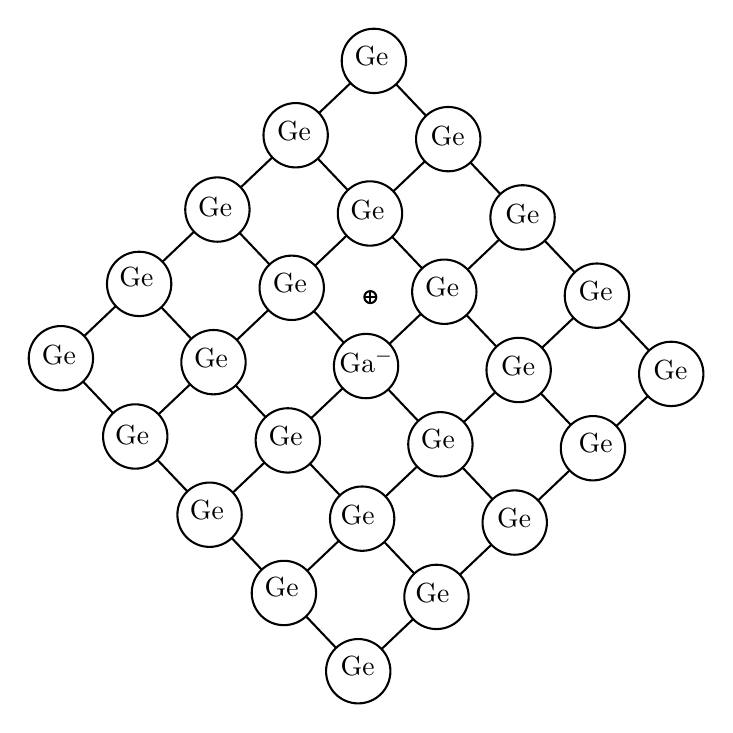
\begin{tikzpicture}[x=0.75pt,y=0.75pt,yscale=-1,xscale=1]
%uncomment if require: \path (0,395); %set diagram left start at 0, and has height of 395

%Shape: Grid [id:dp6807270511623922] 
\draw  [draw opacity=0] (310.17,58.08) -- (453.42,208.89) -- (302.62,352.14) -- (159.36,201.34) -- cycle ; \draw   (345.98,95.78) -- (195.18,239.04)(381.8,133.48) -- (230.99,276.74)(417.61,171.19) -- (266.81,314.44) ; \draw   (272.47,93.9) -- (415.72,244.7)(234.77,129.71) -- (378.02,280.51)(197.06,165.53) -- (340.32,316.33) ; \draw   (310.17,58.08) -- (453.42,208.89) -- (302.62,352.14) -- (159.36,201.34) -- cycle ;
%Shape: Circle [id:dp046063409388742205] 
\draw  [fill={rgb, 255:red, 255; green, 255; blue, 255 }  ,fill opacity=1 ] (143.86,201.34) .. controls (143.86,192.78) and (150.8,185.84) .. (159.36,185.84) .. controls (167.92,185.84) and (174.86,192.78) .. (174.86,201.34) .. controls (174.86,209.9) and (167.92,216.84) .. (159.36,216.84) .. controls (150.8,216.84) and (143.86,209.9) .. (143.86,201.34) -- cycle ;
%Shape: Circle [id:dp5598570457933985] 
\draw  [fill={rgb, 255:red, 255; green, 255; blue, 255 }  ,fill opacity=1 ] (181.56,165.53) .. controls (181.56,156.97) and (188.5,150.03) .. (197.06,150.03) .. controls (205.62,150.03) and (212.56,156.97) .. (212.56,165.53) .. controls (212.56,174.09) and (205.62,181.03) .. (197.06,181.03) .. controls (188.5,181.03) and (181.56,174.09) .. (181.56,165.53) -- cycle ;
%Shape: Circle [id:dp029451512819909986] 
\draw  [fill={rgb, 255:red, 255; green, 255; blue, 255 }  ,fill opacity=1 ] (219.27,129.71) .. controls (219.27,121.15) and (226.2,114.21) .. (234.77,114.21) .. controls (243.33,114.21) and (250.27,121.15) .. (250.27,129.71) .. controls (250.27,138.27) and (243.33,145.21) .. (234.77,145.21) .. controls (226.2,145.21) and (219.27,138.27) .. (219.27,129.71) -- cycle ;
%Shape: Circle [id:dp5621215056634463] 
\draw  [fill={rgb, 255:red, 255; green, 255; blue, 255 }  ,fill opacity=1 ] (256.97,93.9) .. controls (256.97,85.34) and (263.91,78.4) .. (272.47,78.4) .. controls (281.03,78.4) and (287.97,85.34) .. (287.97,93.9) .. controls (287.97,102.46) and (281.03,109.4) .. (272.47,109.4) .. controls (263.91,109.4) and (256.97,102.46) .. (256.97,93.9) -- cycle ;
%Shape: Circle [id:dp6150691897565472] 
\draw  [fill={rgb, 255:red, 255; green, 255; blue, 255 }  ,fill opacity=1 ] (294.67,58.08) .. controls (294.67,49.52) and (301.61,42.58) .. (310.17,42.58) .. controls (318.73,42.58) and (325.67,49.52) .. (325.67,58.08) .. controls (325.67,66.64) and (318.73,73.58) .. (310.17,73.58) .. controls (301.61,73.58) and (294.67,66.64) .. (294.67,58.08) -- cycle ;
%Shape: Circle [id:dp9834237495398297] 
\draw  [fill={rgb, 255:red, 255; green, 255; blue, 255 }  ,fill opacity=1 ] (330.48,95.78) .. controls (330.48,87.22) and (337.42,80.28) .. (345.98,80.28) .. controls (354.54,80.28) and (361.48,87.22) .. (361.48,95.78) .. controls (361.48,104.34) and (354.54,111.28) .. (345.98,111.28) .. controls (337.42,111.28) and (330.48,104.34) .. (330.48,95.78) -- cycle ;
%Shape: Circle [id:dp4811696109046164] 
\draw  [fill={rgb, 255:red, 255; green, 255; blue, 255 }  ,fill opacity=1 ] (366.3,133.48) .. controls (366.3,124.92) and (373.23,117.98) .. (381.8,117.98) .. controls (390.36,117.98) and (397.3,124.92) .. (397.3,133.48) .. controls (397.3,142.05) and (390.36,148.98) .. (381.8,148.98) .. controls (373.23,148.98) and (366.3,142.05) .. (366.3,133.48) -- cycle ;
%Shape: Circle [id:dp31716452119112226] 
\draw  [fill={rgb, 255:red, 255; green, 255; blue, 255 }  ,fill opacity=1 ] (402.11,171.19) .. controls (402.11,162.63) and (409.05,155.69) .. (417.61,155.69) .. controls (426.17,155.69) and (433.11,162.63) .. (433.11,171.19) .. controls (433.11,179.75) and (426.17,186.69) .. (417.61,186.69) .. controls (409.05,186.69) and (402.11,179.75) .. (402.11,171.19) -- cycle ;
%Shape: Circle [id:dp9746450120900616] 
\draw  [fill={rgb, 255:red, 255; green, 255; blue, 255 }  ,fill opacity=1 ] (437.92,208.89) .. controls (437.92,200.33) and (444.86,193.39) .. (453.42,193.39) .. controls (461.98,193.39) and (468.92,200.33) .. (468.92,208.89) .. controls (468.92,217.45) and (461.98,224.39) .. (453.42,224.39) .. controls (444.86,224.39) and (437.92,217.45) .. (437.92,208.89) -- cycle ;
%Shape: Circle [id:dp6515111127767084] 
\draw  [fill={rgb, 255:red, 255; green, 255; blue, 255 }  ,fill opacity=1 ] (292.78,131.6) .. controls (292.78,123.04) and (299.72,116.1) .. (308.28,116.1) .. controls (316.84,116.1) and (323.78,123.04) .. (323.78,131.6) .. controls (323.78,140.16) and (316.84,147.1) .. (308.28,147.1) .. controls (299.72,147.1) and (292.78,140.16) .. (292.78,131.6) -- cycle ;
%Shape: Circle [id:dp4071487594121945] 
\draw  [fill={rgb, 255:red, 255; green, 255; blue, 255 }  ,fill opacity=1 ] (255.08,167.41) .. controls (255.08,158.85) and (262.02,151.91) .. (270.58,151.91) .. controls (279.14,151.91) and (286.08,158.85) .. (286.08,167.41) .. controls (286.08,175.97) and (279.14,182.91) .. (270.58,182.91) .. controls (262.02,182.91) and (255.08,175.97) .. (255.08,167.41) -- cycle ;
%Shape: Circle [id:dp45799565687287735] 
\draw  [fill={rgb, 255:red, 255; green, 255; blue, 255 }  ,fill opacity=1 ] (217.38,203.23) .. controls (217.38,194.67) and (224.32,187.73) .. (232.88,187.73) .. controls (241.44,187.73) and (248.38,194.67) .. (248.38,203.23) .. controls (248.38,211.79) and (241.44,218.73) .. (232.88,218.73) .. controls (224.32,218.73) and (217.38,211.79) .. (217.38,203.23) -- cycle ;
%Shape: Circle [id:dp44147154664981914] 
\draw  [fill={rgb, 255:red, 255; green, 255; blue, 255 }  ,fill opacity=1 ] (179.68,239.04) .. controls (179.68,230.48) and (186.62,223.54) .. (195.18,223.54) .. controls (203.74,223.54) and (210.68,230.48) .. (210.68,239.04) .. controls (210.68,247.6) and (203.74,254.54) .. (195.18,254.54) .. controls (186.62,254.54) and (179.68,247.6) .. (179.68,239.04) -- cycle ;
%Shape: Circle [id:dp9717781572552524] 
\draw  [fill={rgb, 255:red, 255; green, 255; blue, 255 }  ,fill opacity=1 ] (328.59,169.3) .. controls (328.59,160.74) and (335.53,153.8) .. (344.09,153.8) .. controls (352.65,153.8) and (359.59,160.74) .. (359.59,169.3) .. controls (359.59,177.86) and (352.65,184.8) .. (344.09,184.8) .. controls (335.53,184.8) and (328.59,177.86) .. (328.59,169.3) -- cycle ;
%Shape: Circle [id:dp6132423641852609] 
\draw  [fill={rgb, 255:red, 255; green, 255; blue, 255 }  ,fill opacity=1 ] (290.89,205.11) .. controls (290.89,196.55) and (297.83,189.61) .. (306.39,189.61) .. controls (314.95,189.61) and (321.89,196.55) .. (321.89,205.11) .. controls (321.89,213.67) and (314.95,220.61) .. (306.39,220.61) .. controls (297.83,220.61) and (290.89,213.67) .. (290.89,205.11) -- cycle ;
%Shape: Circle [id:dp4060994688976116] 
\draw  [fill={rgb, 255:red, 255; green, 255; blue, 255 }  ,fill opacity=1 ] (253.19,240.93) .. controls (253.19,232.37) and (260.13,225.43) .. (268.69,225.43) .. controls (277.25,225.43) and (284.19,232.37) .. (284.19,240.93) .. controls (284.19,249.49) and (277.25,256.43) .. (268.69,256.43) .. controls (260.13,256.43) and (253.19,249.49) .. (253.19,240.93) -- cycle ;
%Shape: Circle [id:dp11978777626960158] 
\draw  [fill={rgb, 255:red, 255; green, 255; blue, 255 }  ,fill opacity=1 ] (215.49,276.74) .. controls (215.49,268.18) and (222.43,261.24) .. (230.99,261.24) .. controls (239.55,261.24) and (246.49,268.18) .. (246.49,276.74) .. controls (246.49,285.3) and (239.55,292.24) .. (230.99,292.24) .. controls (222.43,292.24) and (215.49,285.3) .. (215.49,276.74) -- cycle ;
%Shape: Circle [id:dp5173906070930463] 
\draw  [fill={rgb, 255:red, 255; green, 255; blue, 255 }  ,fill opacity=1 ] (364.41,207) .. controls (364.41,198.44) and (371.35,191.5) .. (379.91,191.5) .. controls (388.47,191.5) and (395.41,198.44) .. (395.41,207) .. controls (395.41,215.56) and (388.47,222.5) .. (379.91,222.5) .. controls (371.35,222.5) and (364.41,215.56) .. (364.41,207) -- cycle ;
%Shape: Circle [id:dp7739940881746801] 
\draw  [fill={rgb, 255:red, 255; green, 255; blue, 255 }  ,fill opacity=1 ] (326.71,242.81) .. controls (326.71,234.25) and (333.65,227.31) .. (342.21,227.31) .. controls (350.77,227.31) and (357.71,234.25) .. (357.71,242.81) .. controls (357.71,251.37) and (350.77,258.31) .. (342.21,258.31) .. controls (333.65,258.31) and (326.71,251.37) .. (326.71,242.81) -- cycle ;
%Shape: Circle [id:dp9485458234171835] 
\draw  [fill={rgb, 255:red, 255; green, 255; blue, 255 }  ,fill opacity=1 ] (289.01,278.63) .. controls (289.01,270.07) and (295.95,263.13) .. (304.51,263.13) .. controls (313.07,263.13) and (320.01,270.07) .. (320.01,278.63) .. controls (320.01,287.19) and (313.07,294.13) .. (304.51,294.13) .. controls (295.95,294.13) and (289.01,287.19) .. (289.01,278.63) -- cycle ;
%Shape: Circle [id:dp44553437052240064] 
\draw  [fill={rgb, 255:red, 255; green, 255; blue, 255 }  ,fill opacity=1 ] (251.31,314.44) .. controls (251.31,305.88) and (258.25,298.94) .. (266.81,298.94) .. controls (275.37,298.94) and (282.31,305.88) .. (282.31,314.44) .. controls (282.31,323) and (275.37,329.94) .. (266.81,329.94) .. controls (258.25,329.94) and (251.31,323) .. (251.31,314.44) -- cycle ;
%Shape: Circle [id:dp351516880413127] 
\draw  [fill={rgb, 255:red, 255; green, 255; blue, 255 }  ,fill opacity=1 ] (400.22,244.7) .. controls (400.22,236.14) and (407.16,229.2) .. (415.72,229.2) .. controls (424.28,229.2) and (431.22,236.14) .. (431.22,244.7) .. controls (431.22,253.26) and (424.28,260.2) .. (415.72,260.2) .. controls (407.16,260.2) and (400.22,253.26) .. (400.22,244.7) -- cycle ;
%Shape: Circle [id:dp31150061186898537] 
\draw  [fill={rgb, 255:red, 255; green, 255; blue, 255 }  ,fill opacity=1 ] (362.52,280.51) .. controls (362.52,271.95) and (369.46,265.01) .. (378.02,265.01) .. controls (386.58,265.01) and (393.52,271.95) .. (393.52,280.51) .. controls (393.52,289.07) and (386.58,296.01) .. (378.02,296.01) .. controls (369.46,296.01) and (362.52,289.07) .. (362.52,280.51) -- cycle ;
%Shape: Circle [id:dp5931924044042036] 
\draw  [fill={rgb, 255:red, 255; green, 255; blue, 255 }  ,fill opacity=1 ] (324.82,316.33) .. controls (324.82,307.77) and (331.76,300.83) .. (340.32,300.83) .. controls (348.88,300.83) and (355.82,307.77) .. (355.82,316.33) .. controls (355.82,324.89) and (348.88,331.83) .. (340.32,331.83) .. controls (331.76,331.83) and (324.82,324.89) .. (324.82,316.33) -- cycle ;
%Shape: Circle [id:dp8946179633861842] 
\draw  [fill={rgb, 255:red, 255; green, 255; blue, 255 }  ,fill opacity=1 ] (287.12,352.14) .. controls (287.12,343.58) and (294.06,336.64) .. (302.62,336.64) .. controls (311.18,336.64) and (318.12,343.58) .. (318.12,352.14) .. controls (318.12,360.7) and (311.18,367.64) .. (302.62,367.64) .. controls (294.06,367.64) and (287.12,360.7) .. (287.12,352.14) -- cycle ;
%Shape: Circle [id:dp8029888098318514] 
\draw   (305.56,171.89) .. controls (305.56,170.29) and (306.85,169) .. (308.44,169) .. controls (310.04,169) and (311.33,170.29) .. (311.33,171.89) .. controls (311.33,173.48) and (310.04,174.78) .. (308.44,174.78) .. controls (306.85,174.78) and (305.56,173.48) .. (305.56,171.89) -- cycle ;
%Straight Lines [id:da6082337887680658] 
\draw    (305.56,171.89) -- (311.33,171.89) ;
%Straight Lines [id:da29694898334178643] 
\draw    (308.44,169) -- (308.44,174.78) ;

% Text Node
\draw (299.33,49.67) node [anchor=north west][inner sep=0.75pt]   [align=left] {Ge};
% Text Node
\draw (262,85.67) node [anchor=north west][inner sep=0.75pt]   [align=left] {Ge};
% Text Node
\draw (336,88.33) node [anchor=north west][inner sep=0.75pt]   [align=left] {Ge};
% Text Node
\draw (372,125.67) node [anchor=north west][inner sep=0.75pt]   [align=left] {Ge};
% Text Node
\draw (297.33,123.67) node [anchor=north west][inner sep=0.75pt]   [align=left] {Ge};
% Text Node
\draw (407.33,163) node [anchor=north west][inner sep=0.75pt]   [align=left] {Ge};
% Text Node
\draw (443.33,201) node [anchor=north west][inner sep=0.75pt]   [align=left] {Ge};
% Text Node
\draw (224,122.33) node [anchor=north west][inner sep=0.75pt]   [align=left] {Ge};
% Text Node
\draw (186,156.33) node [anchor=north west][inner sep=0.75pt]   [align=left] {Ge};
% Text Node
\draw (148.67,193.67) node [anchor=north west][inner sep=0.75pt]   [align=left] {Ge};
% Text Node
\draw (260,159) node [anchor=north west][inner sep=0.75pt]   [align=left] {Ge};
% Text Node
\draw (333.33,161) node [anchor=north west][inner sep=0.75pt]   [align=left] {Ge};
% Text Node
\draw (222,195) node [anchor=north west][inner sep=0.75pt]   [align=left] {Ge};
% Text Node
\draw (370,199) node [anchor=north west][inner sep=0.75pt]   [align=left] {Ge};
% Text Node
\draw (184,232.33) node [anchor=north west][inner sep=0.75pt]   [align=left] {Ge};
% Text Node
\draw (258,233) node [anchor=north west][inner sep=0.75pt]   [align=left] {Ge};
% Text Node
\draw (331.33,234.33) node [anchor=north west][inner sep=0.75pt]   [align=left] {Ge};
% Text Node
\draw (407.33,236.33) node [anchor=north west][inner sep=0.75pt]   [align=left] {Ge};
% Text Node
\draw (220,268.33) node [anchor=north west][inner sep=0.75pt]   [align=left] {Ge};
% Text Node
\draw (292.67,271) node [anchor=north west][inner sep=0.75pt]   [align=left] {Ge};
% Text Node
\draw (368,272.33) node [anchor=north west][inner sep=0.75pt]   [align=left] {Ge};
% Text Node
\draw (256,305.67) node [anchor=north west][inner sep=0.75pt]   [align=left] {Ge};
% Text Node
\draw (328.67,308.33) node [anchor=north west][inner sep=0.75pt]   [align=left] {Ge};
% Text Node
\draw (292.67,343.67) node [anchor=north west][inner sep=0.75pt]   [align=left] {Ge};
% Text Node
\draw (292,195.67) node [anchor=north west][inner sep=0.75pt]   [align=left] {Ga$\displaystyle ^{-}$};
\end{tikzpicture}
    \caption{Ge中的受主杂质Ga}
    \label{fig:Ge-Ga}
\end{figure}

一个 \ce{Ga}原子占据了原本 \ce{Ge}原子的位置,此原子需要用去4个外层电子与周围的四个 \ce{Ge}原子形成4个共价键;但由于 \ce{Ga}外层仅有3个电子,为了形成4个共价键需要向周围的原子取走一个电子。于是在晶体中形成一个带正电的空穴,而\ce{As}得到一个负电荷,形成\textbf{负电中心}。这种给半导体贡献空穴,并形成负电中心的杂质即称为\textbf{受主杂质}或\textbf{p型杂质}。受主杂质中的空穴得到一定的能量$\Delta E_A$后,价带中的电子进入空穴,事实上形成了脱离束缚的导电空穴,$\Delta E_A$为\textbf{受主杂质电离能},这个电离过程就是\textbf{受主电离}。受主杂质未电离时是中性的,称为\textbf{束缚态}或\textbf{中性态},电离后成为负电中心,称为\textbf{受主离化态}。

空穴被受主杂质束缚时的能量比价带顶$E_v$低$\Delta E_A$。空穴被受主杂质束缚的能量状态称为\textbf{受主能级},记为$E_A$。这样主要依靠空穴导电的半导体称为\textbf{p型半导体}。

\textbf{III族元素}在Ge、Si晶体中是\textbf{受主杂质}。

Si、Ge中的III、V族杂质电离能较小,其受主能级接近价带顶,施主能级接近导带底。通常将这些杂质能级称为\textbf{浅能级},产生浅能级的杂质称为\textbf{浅能级杂质}。

\subsection{浅能级杂质电离能的简单计算}

浅能级杂质电离能较小,电子或空穴受到的束缚很微弱,可以用\textbf{类氢模型}估算杂质电离能。氢原子中电子能量$E_n$为:
\begin{equation}
    E_n=-\frac{m_0q^4}{2(4\pi\varepsilon_0)^2\hslash^2n^2},\quad \text{主量子数}\ n=1,\ 2,\ 3,\cdots
\end{equation}
其中,基态能量$E_1$为:
\begin{equation}
    E_1=-\frac{m_0q^4}{2(4\pi\varepsilon_0)^2\hslash^2}
\end{equation}
氢原子电离态$E_\infty=0$。故氢原子基态电子电离能
\begin{equation}
    E_0=E_\infty-E_1=\frac{m_0q^4}{2(4\pi\varepsilon_0)^2\hslash^2}=13.6\ \mathrm{eV}
\end{equation}

考虑晶体中存在杂质原子,正负电荷处在介电常数\vspace{1ex}$\varepsilon=\varepsilon_0\varepsilon_r$的介质中,则束缚能量将减弱为原来的$\D\frac{1}{\varepsilon_r^2}$。此外电子在晶格周期势场中运动,电子惯性质量$m_0$用有效质量$m_n^*$代替。

修正后的施主杂质电离能表示为:
\begin{equation}
    \Delta E_D=\frac{m_n^*q^4}{2(4\pi\varepsilon_0\varepsilon_r)^2\hslash^2}=\frac{m_n^*}{m_0}\frac{E_0}{\varepsilon_r^2}
\end{equation}

受主杂质电离能为:
\begin{equation}
    \Delta E_A=\frac{m_p^*q^4}{2(4\pi\varepsilon_0\varepsilon_r)^2\hslash^2}=\frac{m_p^*}{m_0}\frac{E_0}{\varepsilon_r^2}
\end{equation}

\subsection{杂质的补偿作用}

半导体中同时存在施主杂质和受主杂质。此时施主杂质和受主杂质有互相抵消的作用,称为杂质的\textbf{补偿作用}。我们用$N_D$表示\textbf{施主杂质浓度},$N_A$表示\textbf{受主杂质浓度},$n$表示导带\textbf{电子浓度},$p$表示价带\textbf{空穴浓度}。

\begin{enumerate}
    \item $N_D\gg N_A$时:

    由于受主能级低于施主能级,施主杂质电子首先跃迁到$N_A$个受主能级上,剩下$N_D-N_A$个电子在施主能级上,杂质电离时跃迁到导带成为导电电子。此时电子浓度$n=N_D-N_A\approx N_D$,半导体为\textbf{n型}。
    \item $N_A\gg N_D$时:

    施主能级上的电子全部跃迁到受主能级后,受主能级还剩$N_A-N_D$个空能级。价带电子跃迁到空能级上,在价带形成导电空穴,空穴浓度为$p=N_A-N_D\approx N_A$,半导体为\textbf{p型}。
\end{enumerate}

利用杂质补偿作用,可以根据需要用\textbf{扩散}或\textbf{离子注入}方法改变半导体的导电类型。若出现$N_D\approx N_A$,此时施主电子刚好填充受主能级,虽然杂质很多,却无法向导带和价带提供电子和空穴,这种现象称为\textbf{杂质高度补偿}。

\section{缺陷、位错能级}

\subsection{点缺陷}

一定温度下,晶格原子会在平衡位置附近作振动运动,此时一部分原子获得足够的能量,克服周围原子对其束缚,挤入其他原子间隙,形成\textbf{间隙原子},原来的位置便会成为\textbf{空位}。此时间隙原子与空位成对出现,成为\textbf{弗伦克尔缺陷}。而只在晶体内形成空位而无间隙原子,则称为\textbf{肖特基缺陷}。间隙原子与空位不断产生和复合,形成平衡浓度。上述两种由温度决定的点缺陷称为\textbf{热缺陷}。原子需较大的能量才能挤入间隙位置,然而其迁移的激活能很小,因此晶体中空位比间隙原子多得多。空位是常见的点缺陷。

\subsection{位错}

\textbf{位错}是半导体的一种缺陷。在晶体的棱位错周围,晶格会发生畸变。






